% Options for packages loaded elsewhere
\PassOptionsToPackage{unicode}{hyperref}
\PassOptionsToPackage{hyphens}{url}
%
\documentclass[
  ignorenonframetext,
]{beamer}
\usepackage{pgfpages}
\setbeamertemplate{caption}[numbered]
\setbeamertemplate{caption label separator}{: }
\setbeamercolor{caption name}{fg=normal text.fg}
\beamertemplatenavigationsymbolsempty
% Prevent slide breaks in the middle of a paragraph
\widowpenalties 1 10000
\raggedbottom
\setbeamertemplate{part page}{
  \centering
  \begin{beamercolorbox}[sep=16pt,center]{part title}
    \usebeamerfont{part title}\insertpart\par
  \end{beamercolorbox}
}
\setbeamertemplate{section page}{
  \centering
  \begin{beamercolorbox}[sep=12pt,center]{part title}
    \usebeamerfont{section title}\insertsection\par
  \end{beamercolorbox}
}
\setbeamertemplate{subsection page}{
  \centering
  \begin{beamercolorbox}[sep=8pt,center]{part title}
    \usebeamerfont{subsection title}\insertsubsection\par
  \end{beamercolorbox}
}
\AtBeginPart{
  \frame{\partpage}
}
\AtBeginSection{
  \ifbibliography
  \else
    \frame{\sectionpage}
  \fi
}
\AtBeginSubsection{
  \frame{\subsectionpage}
}
\usepackage{lmodern}
\usepackage{amssymb,amsmath}
\usepackage{ifxetex,ifluatex}
\ifnum 0\ifxetex 1\fi\ifluatex 1\fi=0 % if pdftex
  \usepackage[T1]{fontenc}
  \usepackage[utf8]{inputenc}
  \usepackage{textcomp} % provide euro and other symbols
\else % if luatex or xetex
  \usepackage{unicode-math}
  \defaultfontfeatures{Scale=MatchLowercase}
  \defaultfontfeatures[\rmfamily]{Ligatures=TeX,Scale=1}
\fi
\usetheme[]{Madrid}
\usecolortheme{lily}
% Use upquote if available, for straight quotes in verbatim environments
\IfFileExists{upquote.sty}{\usepackage{upquote}}{}
\IfFileExists{microtype.sty}{% use microtype if available
  \usepackage[]{microtype}
  \UseMicrotypeSet[protrusion]{basicmath} % disable protrusion for tt fonts
}{}
\makeatletter
\@ifundefined{KOMAClassName}{% if non-KOMA class
  \IfFileExists{parskip.sty}{%
    \usepackage{parskip}
  }{% else
    \setlength{\parindent}{0pt}
    \setlength{\parskip}{6pt plus 2pt minus 1pt}}
}{% if KOMA class
  \KOMAoptions{parskip=half}}
\makeatother
\usepackage{xcolor}
\IfFileExists{xurl.sty}{\usepackage{xurl}}{} % add URL line breaks if available
\IfFileExists{bookmark.sty}{\usepackage{bookmark}}{\usepackage{hyperref}}
\hypersetup{
  pdftitle={Program Evaluation (Causal Inference) 1: Introduction},
  pdfauthor={Instructor: Yuta Toyama},
  hidelinks,
  pdfcreator={LaTeX via pandoc}}
\urlstyle{same} % disable monospaced font for URLs
\newif\ifbibliography
\usepackage{graphicx}
\makeatletter
\def\maxwidth{\ifdim\Gin@nat@width>\linewidth\linewidth\else\Gin@nat@width\fi}
\def\maxheight{\ifdim\Gin@nat@height>\textheight\textheight\else\Gin@nat@height\fi}
\makeatother
% Scale images if necessary, so that they will not overflow the page
% margins by default, and it is still possible to overwrite the defaults
% using explicit options in \includegraphics[width, height, ...]{}
\setkeys{Gin}{width=\maxwidth,height=\maxheight,keepaspectratio}
% Set default figure placement to htbp
\makeatletter
\def\fps@figure{htbp}
\makeatother
\setlength{\emergencystretch}{3em} % prevent overfull lines
\providecommand{\tightlist}{%
  \setlength{\itemsep}{0pt}\setlength{\parskip}{0pt}}
\setcounter{secnumdepth}{-\maxdimen} % remove section numbering
\usetheme{Madrid}        
\setbeamertemplate{navigation symbols}{} 
\setbeamertemplate{footline}[frame number] 
\setbeamercolor{page number in head/foot}{fg=black}

\setbeamersize{text margin left=3mm,text margin right=3mm}
\useoutertheme[footline=empty,subsection=false]{miniframes} 
\usecolortheme{lily}
\setbeamerfont{frametitle}{size=\large}
\setbeamertemplate{items}[default]

\setlength{\leftmargini}{14pt}

%% change fontsize of R code
\let\oldShaded\Shaded
\let\endoldShaded\endShaded
\renewenvironment{Shaded}{\footnotesize\oldShaded}{\endoldShaded}

%% change fontsize of output
\let\oldverbatim\verbatim
\let\endoldverbatim\endverbatim
\renewenvironment{verbatim}{\footnotesize\oldverbatim}{\endoldverbatim}

\title{Program Evaluation (Causal Inference) 1: Introduction}
\author{Instructor: Yuta Toyama}
\date{Last updated: 2020-05-10}

\begin{document}
\frame{\titlepage}

\hypertarget{introduction}{%
\section{Introduction}\label{introduction}}

\begin{frame}{Introduction}
\protect\hypertarget{introduction-1}{}
\begin{itemize}
\item
  Program Evaluation, or Causal Inference

  \begin{itemize}
  \item
    Estimation of ``treatment effect'' of some intervention (typically
    binary)
  \item
    Example:

    \begin{itemize}
    \tightlist
    \item
      effects of job training on wage
    \item
      effects of advertisement on purchase behavior
    \item
      effects of distributing mosquito net on children's school
      attendance
    \end{itemize}
  \end{itemize}
\item
  Difficulty: treatment is \textbf{endogenous decision}

  \begin{itemize}
  \item
    selection bias, omitted variable bias.
  \item
    especially in observational data (in comparison with experimental
    data)
  \end{itemize}
\end{itemize}
\end{frame}

\begin{frame}{Overview}
\protect\hypertarget{overview}{}
\begin{itemize}
\item
  Introduce Rubin's causal model (potential outcome framework)

  \begin{itemize}
  \tightlist
  \item
    Generalization of the linear regression model: Nonparametric
  \end{itemize}
\item
  Solutions to the selection bias

  \begin{enumerate}
  \item
    Randomized control trial (today)
  \item
    Matching (today)
  \item
    Instrumental Variable Estimation (today)
  \item
    Difference-in-differences (next week)
  \item
    Regression Discontinuity Design (week after next)
  \end{enumerate}
\end{itemize}
\end{frame}

\begin{frame}{Reference}
\protect\hypertarget{reference}{}
\begin{itemize}
\item
  Angrist and Pischke:

  \begin{itemize}
  \item
    Mostly harmless econometrics : advanced undergraduate to graduate
    students
  \item
    Mastering Metrics: good for undergraduate students after taking
    econometrics course.
  \end{itemize}
\item
  Ito: Data Bunseki no Chikara (in Japanese)
\end{itemize}
\end{frame}

\hypertarget{framework}{%
\section{Framework}\label{framework}}

\begin{frame}{Framework}
\protect\hypertarget{framework-1}{}
\begin{itemize}
\item
  \(Y_{i}\): observed outcome for person \(i\)
\item
  \(D_{i}\): treatment status \[D_{i}=\begin{cases}
  1 & treated\ (treatment\ group)\\
  0 & not\ treated\ (control\ group)
  \end{cases}\]
\item
  Define \emph{potential outcomes}

  \begin{itemize}
  \item
    \(Y_{1i}\): outcome for \(i\) when she is treated (treatment group)
  \item
    \(Y_{0i}\): outcome for \(i\) when she is not treated (control
    group)
  \end{itemize}
\item
  With this, we can write \[\begin{aligned}
  Y_{i} & =D_{i}Y_{1i}+(1-D_{i})Y_{0i}\\
   & =\begin{cases}
  Y_{1i} & if\ D_{i}=1\\
  Y_{0i} & if\ D_{i}=0
  \end{cases}\end{aligned}\]
\end{itemize}
\end{frame}

\begin{frame}{Two Key points}
\protect\hypertarget{two-key-points}{}
\begin{itemize}
\item
  Point 1: Fundamental problem of program evaluation

  \begin{itemize}
  \item
    We can observe \((Y_{i},D_{i})\), but never observe \(Y_{0i}\) and
    \(Y_{1i}\) \textbf{simultaneously}.
  \item
    \textbf{Counterfactual} outcome.
  \end{itemize}
\item
  Point 2: Stable Unit Treatment Value Assumption (SUTVA)

  \begin{itemize}
  \item
    Treatment effect for a person does \textbf{not depend on the
    treatment status of other people.}
  \item
    Rules out externality / general equilibrium effects.

    \begin{itemize}
    \tightlist
    \item
      Ex: If everyone takes the job training, the equilibrium wage would
      change, which affects the individual outcome.
    \end{itemize}
  \end{itemize}
\end{itemize}
\end{frame}

\begin{frame}{Parameters of Interest}
\protect\hypertarget{parameters-of-interest}{}
\begin{itemize}
\item
  Define the individual treatment effect \(Y_{1i}-Y_{0i}\)

  \begin{itemize}
  \tightlist
  \item
    Key: allowing for heterogenous effects across people
  \end{itemize}
\item
  Individual treatment effect cannot be identified due to the
  fundamental problem.
\item
  Instead, we focus on the average effects

  \begin{itemize}
  \item
    Average treatment effect: \(ATE=E[Y_{1i}-Y_{0i}]\)
  \item
    Average treatment effect on treated:
    \(ATT=E[Y_{1i}-Y_{0i}|D_{i}=1]\)
  \item
    Average treatment effect on untreated:
    \(ATT=E[Y_{1i}-Y_{0i}|D_{i}=0]\)
  \item
    Average treatment effect conditional on covariates \(X_{i}\):
    \(ATE(x)=E[Y_{1i}-Y_{0i}|D_{i}=1,X_{i}=x]\)
  \end{itemize}
\end{itemize}
\end{frame}

\begin{frame}{Relation to Regression Analysis}
\protect\hypertarget{relation-to-regression-analysis}{}
\begin{itemize}
\item
  Assume that

  \begin{enumerate}
  \item
    linear (parametric) structure in \(Y_{0i}\), and
  \item
    constant (homogenous) treatment effect, \[\begin{aligned}
    Y_{0i} & =\beta_{0}+\epsilon_{i}\\
    Y_{1i}-Y_{0i} & =\beta_{1}\end{aligned}\]
  \end{enumerate}
\item
  You will have \[Y_{i}=\beta_{0}+\beta_{1}D_{i}+\epsilon_{i}\]
\item
  Program evaluation framework is nonparametric in nature.

  \begin{itemize}
  \tightlist
  \item
    Though, in practice, estimation of treatment effect relies on a
    parametric specification.
  \end{itemize}
\end{itemize}
\end{frame}

\begin{frame}{Selection Bias}
\protect\hypertarget{selection-bias}{}
\begin{itemize}
\item
  Consider the comparison of average outcomes between treatment and
  control group
\item
  Does this tell you average treatment effect? No in general!
  \[\begin{aligned}
  \underbrace{E[Y_{i}|D_{i}=1]-E[Y_{i}|D_{i}=0]}_{simple\ comparison}= & E[Y_{1i}|D_{i}=1]-E[Y_{0i}|D_{i}=0]\\
  = & \underbrace{E[Y_{1i}-Y_{0i}|D_{i}=1]}_{ATT}\\
   & +\underbrace{E[Y_{0i}|D_{i}=1]-E[Y_{0i}|D_{i}=0]}_{selection\ bias}\end{aligned}\]
\item
  The bias term \(E[Y_{0i}|D_{i}=1]-E[Y_{0i}|D_{i}=0]\)

  \begin{itemize}
  \item
    not zero in general: Those who are taking the job training
    \textbf{would do a good job even without job training}
  \item
    Cannot observe \(E[Y_{0i}|D_{i}=1]\): the outcome of people in
    treatment group when they are NOT treated (counterfactual).
  \end{itemize}
\end{itemize}
\end{frame}

\begin{frame}{Solutions}
\protect\hypertarget{solutions}{}
\begin{itemize}
\item
  The core of program evaluation is how to identify (estimate) the
  treatment effect parameters.
\item
  Randomized Control Trial (A/B test):

  \begin{itemize}
  \tightlist
  \item
    Assign treatment \(D_{i}\) randomly
  \end{itemize}
\item
  Matching (regression):

  \begin{itemize}
  \tightlist
  \item
    Using observed characteristics of individuals to control for
    selection bias
  \end{itemize}
\item
  Instrumental variable

  \begin{itemize}
  \tightlist
  \item
    Use the variable that affects treatment status but is not correlated
    to the outcome
  \end{itemize}
\item
  Difference-in-differences

  \begin{itemize}
  \tightlist
  \item
    Use the panel data to control for individual heterogeneity by fixed
    effects.
  \end{itemize}
\item
  Regression Discontinuity Design

  \begin{itemize}
  \tightlist
  \item
    Exploit the randomness around the thresholds.
  \end{itemize}
\item
  Others: Bound approach, synthetic control method, regression kink
  design, etc..
\end{itemize}
\end{frame}

\hypertarget{rct}{%
\section{RCT}\label{rct}}

\begin{frame}{What is RCT ?}
\protect\hypertarget{what-is-rct}{}
\begin{itemize}
\item
  RCT: Randomized Controlled Trial
\item
  Measure the effect of ``treatment'' by

  \begin{enumerate}
  \item
    randomly assigning treatment to a particular group (treatment group)
  \item
    measure outcomes of subjects in both treatment and ``control''
    group.
  \item
    the difference of outcomes between these two groups is ``treatment''
    effect.
  \end{enumerate}
\item
  Starts with clinical trial: measure the effects of medicine.
\end{itemize}
\end{frame}

\begin{frame}{Example from Development Economics}
\protect\hypertarget{example-from-development-economics}{}
\begin{itemize}
\item
  Esther Duflo ``Social experiments to fight poverty''

  \begin{itemize}
  \tightlist
  \item
    \url{https://www.ted.com/talks/esther_duflo_social_experiments_to_fight_poverty?language=en}
  \end{itemize}
\end{itemize}
\end{frame}

\begin{frame}{Framework}
\protect\hypertarget{framework-2}{}
\begin{itemize}
\item
  Key assumption: Treatment \(D_{i}\) is independent with potential
  outcomes \((Y_{0i},Y_{1i})\) \[D_{i}\perp(Y_{0i},Y_{1i})\]
\item
  Under this assumption, \[\begin{aligned}
  E[Y_{1i}|D_{i} & =1]=E[Y_{1i}|D_{i}=0]=E[Y_{1i}]\\
  E[Y_{0i}|D_{i} & =1]=E[Y_{0i}|D_{i}=0]=E[Y_{0i}]\end{aligned}\]
\item
  The sample selection does not exist! Thus, \[\begin{aligned}
  \underbrace{E[Y_{i}|D_{i}=1]-E[Y_{i}|D_{i}=0]}_{simple\ comparison}= & \underbrace{E[Y_{1i}-Y_{0i}|D_{i}=1]}_{ATT}\end{aligned}\]
\item
  Difference of the sample average is consistent estimator for the ATT
  \[\frac{\frac{1}{N}\sum_{i=1}^{N}Y_{i}\cdot\mathbf{1}\{D_{i}=1\}}{\frac{1}{N}\sum_{i=1}^{N}\mathbf{1}\{D_{i}=1\}}-\frac{\frac{1}{N}\sum_{i=1}^{N}Y_{i}\cdot\mathbf{1}\{D_{i}=0\}}{\frac{1}{N}\sum_{i=1}^{N}\mathbf{1}\{D_{i}=0\}}\]
\end{itemize}
\end{frame}

\begin{frame}{Example: RAND Health Insurance Experiment (HIE)}
\protect\hypertarget{example-rand-health-insurance-experiment-hie}{}
\begin{itemize}
\item
  Taken from Angrist and Pischke (2014, Sec 1.1)
\item
  1974-1982, 3958 people, age 14-61
\item
  Randomly assigned to one of 14 insurance plans.

  \begin{itemize}
  \item
    No insurance premium
  \item
    Different provisions related to cost sharing
  \end{itemize}
\item
  4 categories

  \begin{itemize}
  \item
    Free
  \item
    Co-insurance: Pay 25-50\% of costs
  \item
    Deductible: Pay 95\% of costs, up to \$150 per person (\$450 per
    family)
  \item
    Catastrophic coverage: 95\% of health costs. No upper limit.
    Approximate ``no insurance''
  \end{itemize}
\end{itemize}
\end{frame}

\begin{frame}{First step: Balance Check}
\protect\hypertarget{first-step-balance-check}{}
\begin{figure}
\centering
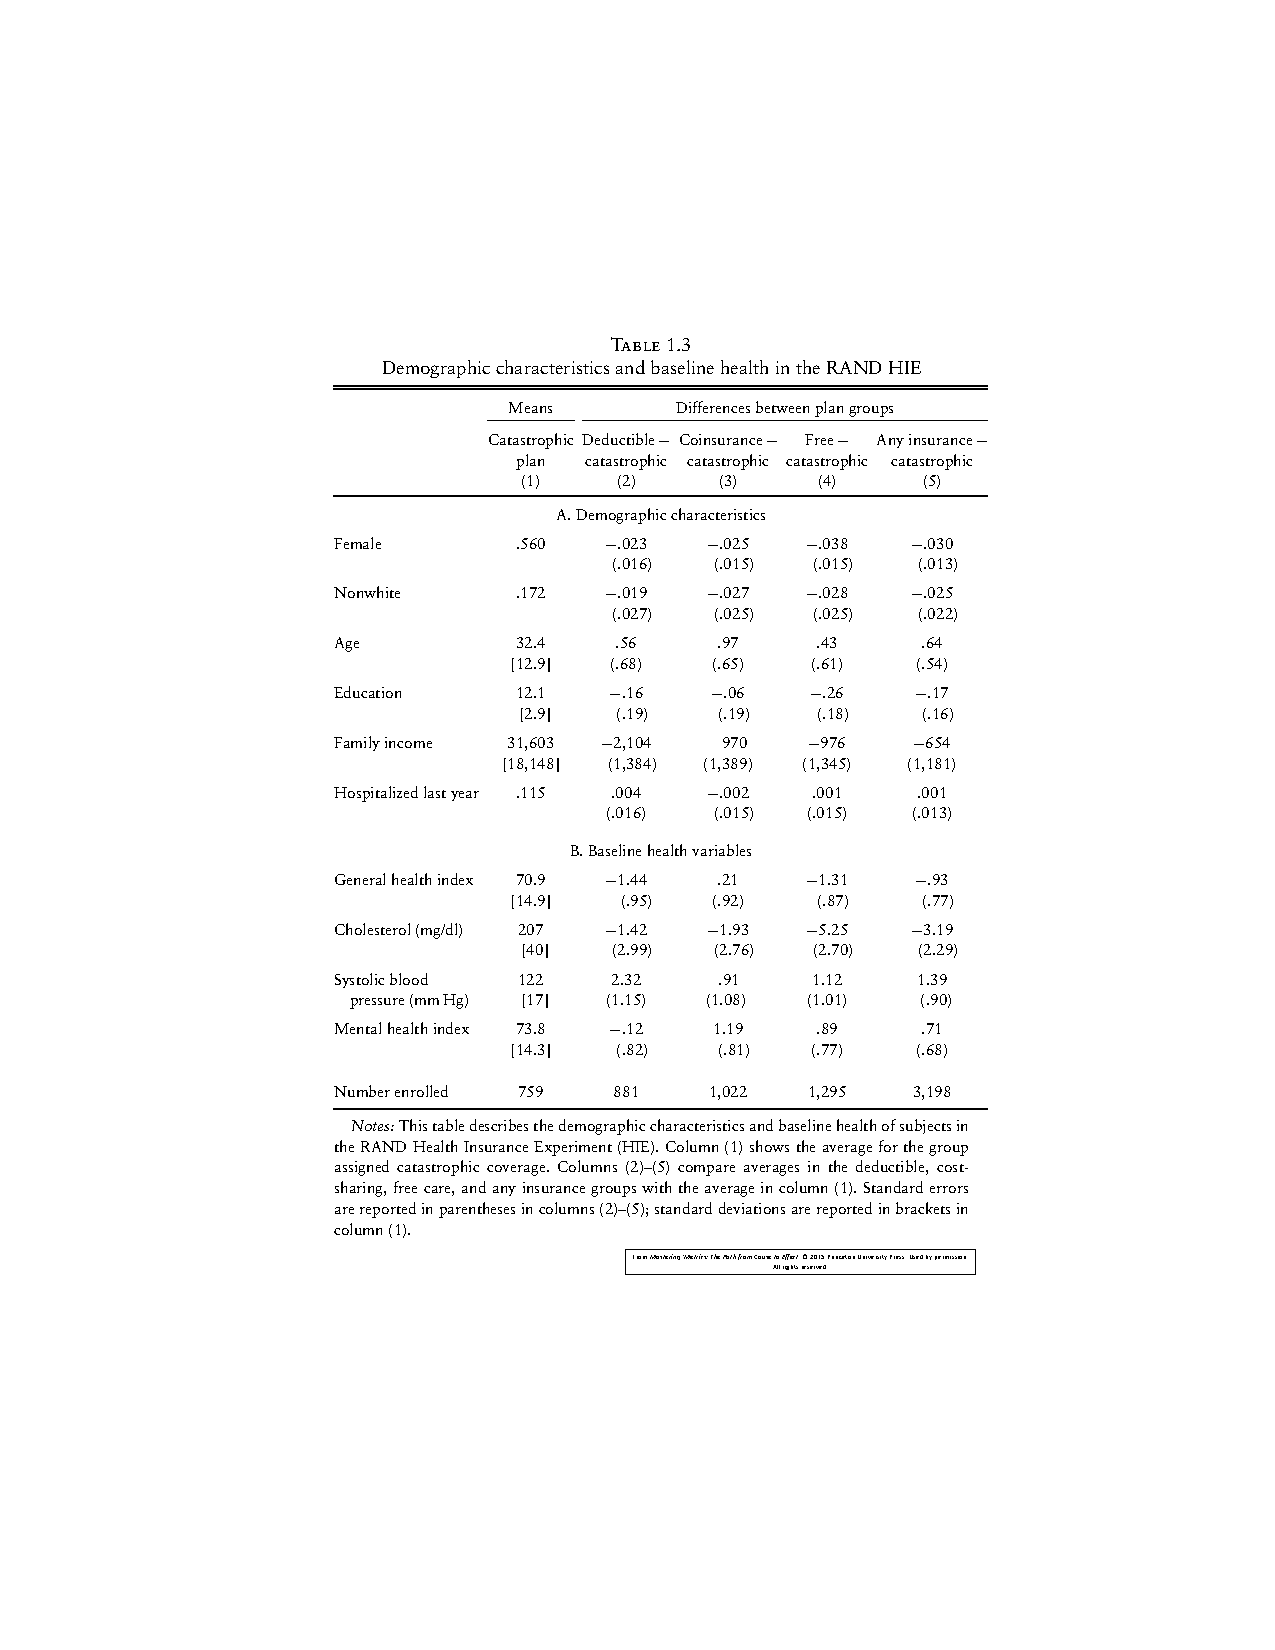
\includegraphics{figure_table/MMtbl13.pdf}
\caption{image}
\end{figure}

\begin{itemize}
\item
  Differences in demographic characteristics \& baseline health are
  statistically insignificant
\item
  Assignment of health insurance plans is indeed random!
\end{itemize}
\end{frame}

\begin{frame}{Results of RAND HIE}
\protect\hypertarget{results-of-rand-hie}{}
\begin{figure}
\centering
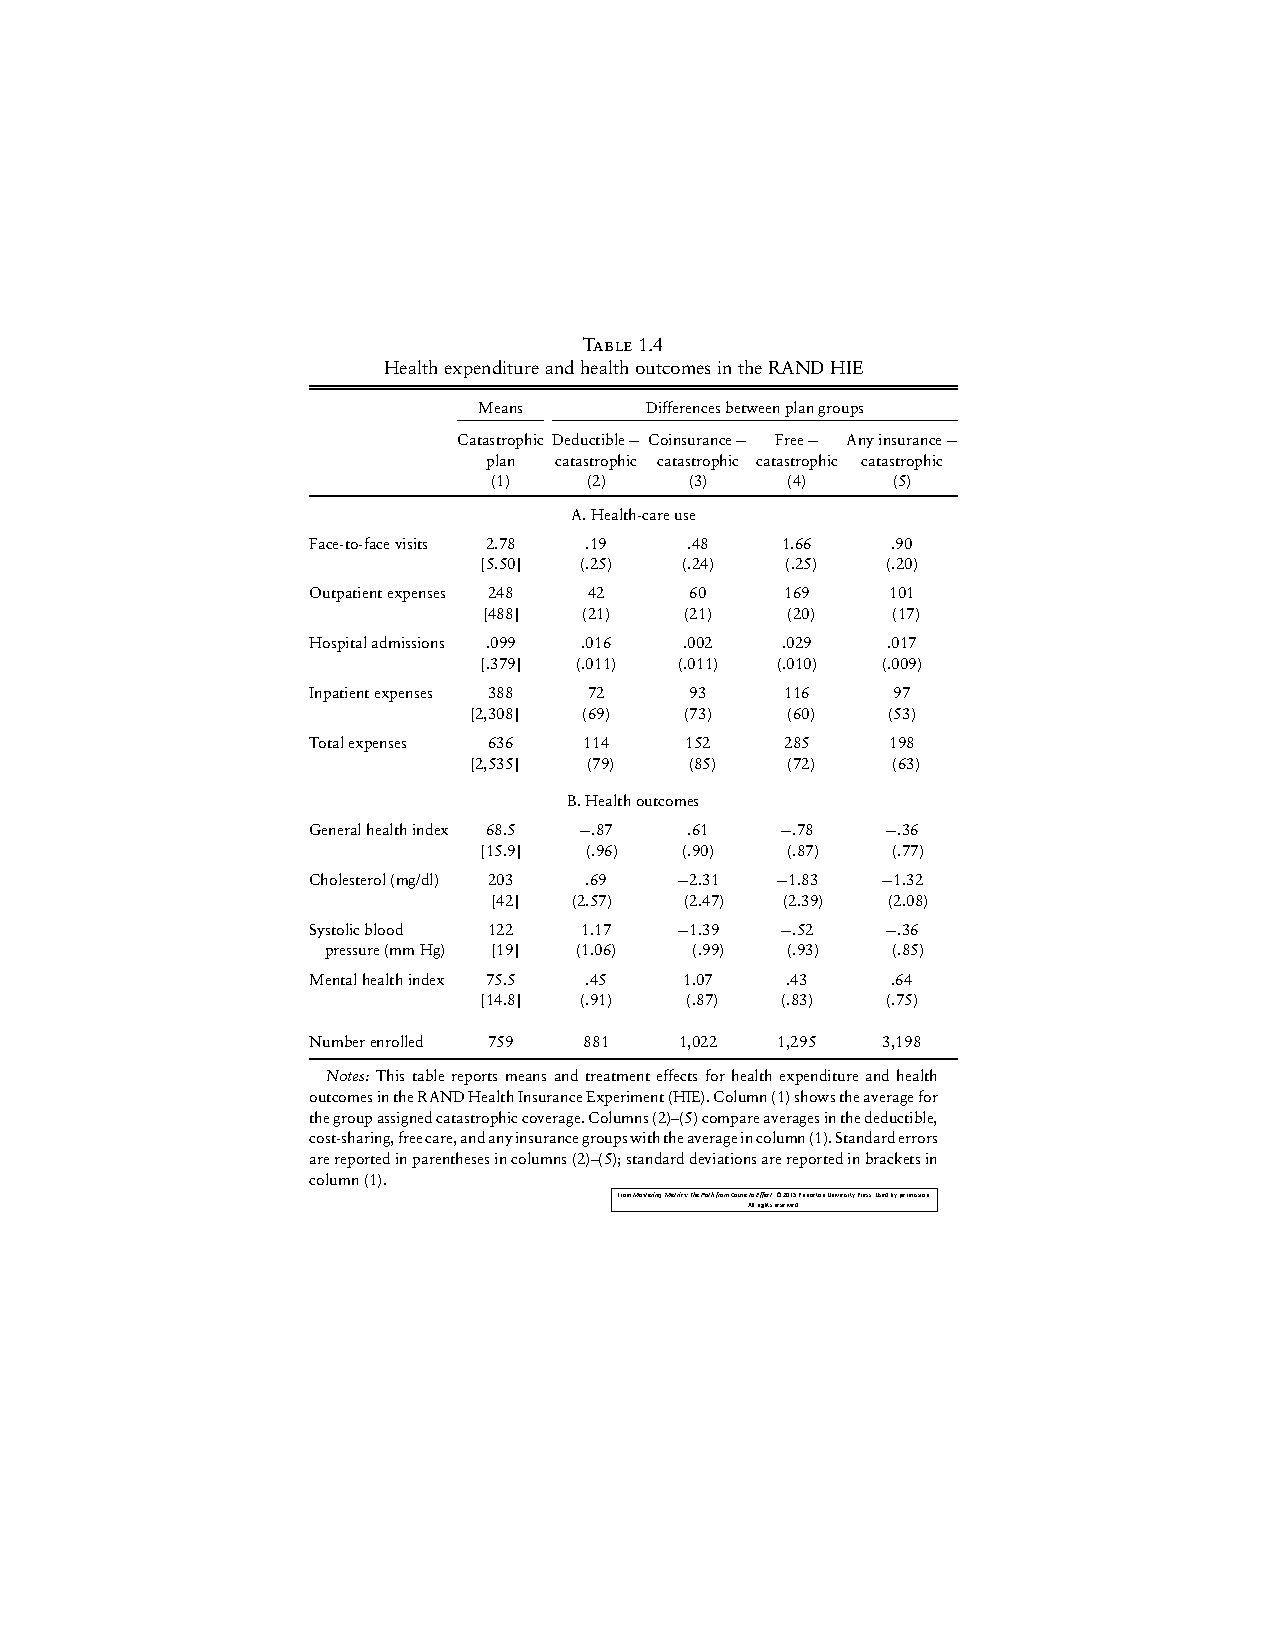
\includegraphics{figure_table/MMtbl14.pdf}
\caption{image}
\end{figure}

\begin{itemize}
\item
  HI increases health spending (Panel A)
\item
  But, HI has no statistically significant effect on health outcomes
\end{itemize}
\end{frame}

\hypertarget{matching}{%
\section{Matching}\label{matching}}

\begin{frame}{Matching}
\protect\hypertarget{matching-1}{}
\begin{itemize}
\item
  Idea: Compare \textbf{individuals with the same characteristics \(X\)}
  across treatment and control groups
\item
  Let \(X_{i}\) denote the observed characteristics: age, income,
  education, race, etc...
\item
  Assumption 1: \[D_{i}\perp(Y_{0i},Y_{1i})\left|X_{i}\right.\]

  \begin{itemize}
  \item
    Conditional on \(X_{i}\), no selection bias.
  \item
    Selection on observables assumption / ignorability
  \end{itemize}
\item
  Assumption 2: Overlap assumption
  \[P(D_{i}=1|X_{i}=x)\in(0,1)\ \forall x\]

  \begin{itemize}
  \tightlist
  \item
    Given \(x\), we should be able to observe people from both control
    and treatment group.
  \end{itemize}
\end{itemize}
\end{frame}

\begin{frame}{Identification}
\protect\hypertarget{identification}{}
\begin{itemize}
\item
  The assumption implies that \[\begin{aligned}
  E[Y_{1i}|D_{i} & =1,X_{i}]=E[Y_{1i}|D_{i}=0,X_{i}]=E[Y_{1i}|X_{i}]\\
  E[Y_{0i}|D_{i} & =1,X_{i}]=E[Y_{0i}|D_{i}=0,X_{i}]=E[Y_{0i}|X_{i}]\end{aligned}\]
\item
  The \(ATT\) for \(X_{i}=x\) is given by \[\begin{aligned}
  E[Y_{1i}-Y_{0i}|D_{i}=1,X_{i}] & =E[Y_{1i}|D_{i}=1,X_{i}]-E[Y_{0i}|D_{i}=1,X_{i}]\\
   & =E[Y_{i}|D_{i}=1,X_{i}]-E[Y_{0i}|D_{i}=0,X_{i}]\\
   & =\underbrace{E[Y_{i}|D_{i}=1,X_{i}]}_{avg\ with\ X_{i}\ in\ treatment}-\underbrace{E[Y_{i}|D_{i}=0,X_{i}]}_{avg\ with\ X_{i}\ in\ control}\end{aligned}\]
\item
  The components in the last line are identified (can be estimated).
\item
  Intuition: Comparing the outcome across control and treatment groups
  after conditioning on \(X_{i}\)
\end{itemize}
\end{frame}

\begin{frame}{ATT and ATE}
\protect\hypertarget{att-and-ate}{}
\begin{itemize}
\item
  ATT is given by \[\begin{aligned}
  ATT & =E[Y_{1i}-Y_{0i}|D_{i}=1]\\
   & =\int E[Y_{1i}-Y_{0i}|D_{i}=1,X_{i}=x]f_{X_{i}}(x|D_{i}=1)dx\\
   & =E[Y_{i}|D_{i}=1]-\int\left(E[Y_{i}|D_{i}=0,X_{i}=x]\right)f_{X_{i}}(x|D_{i}=1)\end{aligned}\]
\item
  ATE is \[\begin{aligned}
  ATE= & E[Y_{1i}-Y_{0i}]\\
  = & \int E[Y_{1i}-Y_{0i}|X_{i}=x]f_{X_{i}}(x)dx\\
  = & \int E[Y_{i}|D_{i}=1,X_{i}=x]f_{X_{i}}(x)dx\\
  = & +\int E[Y_{i}|D_{i}=0,X_{i}=x]f_{X_{i}}(x)dx\end{aligned}\]
\end{itemize}
\end{frame}

\begin{frame}{Estimation Methods}
\protect\hypertarget{estimation-methods}{}
\begin{itemize}
\item
  We need to estimate \(E[Y_{i}|D_{i}=1,X_{i}=x]\) and
  \(E[Y_{i}|D_{i}=0,X_{i}=x]\)
\item
  Several ways to implement the above idea
\item
  Regression: Nonparametric and Parametric
\item
  Nearest neighborhood matching
\item
  Propensity Score Matching: Skipped
\end{itemize}

Regression, or Analogue Approach

\begin{itemize}
\item
  Let \(\hat{\mu}_{k}(x)\) be an estimator of
  \(\mu_{k}(x)=E[Y_{i}|D_{i}=k,X_{i}=x]\) for \(k\in\{0,1\}\)
\item
  The analog estimators are \[\begin{aligned}
  \hat{ATE} & =\frac{1}{N}\sum_{i=1}^{N}\hat{\mu}_{1}(X_{i})-\hat{\mu}_{0}(X_{i})\\
  \hat{ATT} & =\frac{N^{-1}\sum_{i=1}^{N}D_{i}(Y_{i}-\hat{\mu}_{0}(X_{i}))}{N^{-1}\sum_{i=1}^{N}D_{i}}\end{aligned}\]
\item
  How to estimate \(\mu_{k}(x)=E[Y_{i}|D_{i}=k,X_{i}=x]\) ?
\end{itemize}
\end{frame}

\begin{frame}{Nonparametric Estimation}
\protect\hypertarget{nonparametric-estimation}{}
\begin{itemize}
\item
  Suppose that \(X_{i}\in\{x_{1},\cdots,x_{K}\}\) is discrete with small
  \(K\)

  \begin{itemize}
  \tightlist
  \item
    Ex: two demographic characteristics (male/female, white/non-white).
    \(K=4\)
  \end{itemize}
\item
  Then, a nonparametric binning estimator is
  \[\hat{\mu}_{k}(x)=\frac{\sum_{i=1}^{N}\mathbf{1}\{D_{i}=k,X_{i}=x\}Y_{i}}{\sum_{i=1}^{N}\mathbf{1}\{D_{i}=k,X_{i}=x\}}\]
\item
  Here, I do not put any parametric assumption on
  \(\mu_{k}(x)=E[Y_{i}|D_{i}=k,X_{i}=x]\).
\item
  Issue: Poor performance if \(K\) is large due to many covariates

  \begin{itemize}
  \tightlist
  \item
    \textbf{curse of dimensionality}
  \end{itemize}
\item
  If \(X\) can take continuum value, you can use kernel regression.
\end{itemize}
\end{frame}

\begin{frame}{Parametric Estimation, or going back to linear regression}
\protect\hypertarget{parametric-estimation-or-going-back-to-linear-regression}{}
\begin{itemize}
\item
  If you put parametric assumption such as \[\begin{aligned}
  E[Y_{i}|D_{i}=0,X_{i}=x] & =\beta'x_{i}\\
  E[Y_{i}|D_{i}=1,X_{i}=x] & =\beta'x_{i}+\tau_{0}\end{aligned}\] then,
  you will have a model \[y_{i}=\beta'x_{i}+\tau D_{i}+\epsilon_{i}\]
\item
  You can think the matching estimator as controlling for omitted
  variable bias by adding (many) covariates (control variables)
  \(x_{i}\).
\item
  This is one reason why matching estimator may not be preferred in
  empirical research.

  \begin{itemize}
  \tightlist
  \item
    Remember: Controlling for those covariates is of course important.
    This can be combined with other empirical strategies (IV, DID, etc).
  \end{itemize}
\end{itemize}
\end{frame}

\begin{frame}{\(M-\)Nearest Neighborhood Matching}
\protect\hypertarget{m-nearest-neighborhood-matching}{}
\begin{itemize}
\item
  Fine the counterpart in other group that is close to me.
\item
  Define \(\hat{y}_{i}(0)\) and \(\hat{y}_{i}(1)\) be the estimator for
  (hypothetical) outcomes when treated and not treated.
  \[\hat{y}_{i}(0)=\begin{cases}
  y_{i} & if\ D_{i}=0\\
  \frac{1}{M}\sum_{j\in L_{M}(i)}y_{j} & if\ D_{i}=1
  \end{cases}\]
\item
  \(L_{M}(i)\) is the set of \(M\) individuals in the opposite group who
  are ``close'' to individual \(i\)

  \begin{itemize}
  \item
    Closeness is defined as the distance between \(X_{i}\) and \(X_{j}\)
  \item
    There are several ways to define the distance. For example,
    \[dist(X_{i},X_{j})=||X_{i}-X_{j}||^{2}\]
  \end{itemize}
\item
  You need to choose (1) \(M\) and (2) the measure of distance to
  implement this.
\item
  R has several packages for this.
\end{itemize}
\end{frame}

\hypertarget{going-forward}{%
\section{Going Forward}\label{going-forward}}

\begin{frame}{Other Approaches}
\protect\hypertarget{other-approaches}{}
\begin{itemize}
\item
  Instrumental Variable: same idea.

  \begin{itemize}
  \tightlist
  \item
    IV estimation in program evaluation framework involves with the
    argument of local average treatment effect (LATE), which is beyond
    the scope of this course.
  \end{itemize}
\item
  Difference in differences (week 14)
\item
  Regression discontinuity design (week 15)
\end{itemize}
\end{frame}

\end{document}
